
%%%%%%%%%%%%%%
%%% DESIGN %%%
%%%%%%%%%%%%%%

\chapter{Design}

WHY we design this

HOW we design this

WHAT this chapter reports

Lorem ipsum dolor sit amet, consectetuer adipiscing elit, sed diam nonummy nibh euismod tincidunt ut laoreet dolore magna aliquam erat volutpat. Ut wisi enim ad minim veniam, quis nostrud exerci tation ullamcorper suscipit lobortis nisl ut aliquip ex ea commodo consequat. Duis autem vel eum iriure dolor in hendrerit in vulputate velit esse molestie consequat, vel illum dolore eu feugiat nulla facilisis at vero eros et accumsan et iusto odio dignissim qui blandit praesent luptatum zzril delenit augue duis dolore te feugait nulla facilisi. Nam liber tempor cum soluta nobis eleifend option congue nihil imperdiet doming id quod mazim placerat facer possim assum. Typi non habent claritatem insitam; est usus legentis in iis qui facit eorum claritatem. Investigationes demonstraverunt lectores legere me lius quod ii legunt saepius. Claritas est etiam processus dynamicus, qui sequitur mutationem consuetudium lectorum. Mirum est notare quam littera gothica, quam nunc putamus parum claram, anteposuerit litterarum formas humanitatis per seacula quarta decima et quinta decima. Eodem modo typi, qui nunc nobis videntur parum clari, fiant sollemnes in futurum.

% Design principles, inspiration, methodology

%The thesis investigated here is that using tabletops as basic Input/Output peripherals for other computing devices will help their adoption by the masses.
%A user should be able to transfer the display of his/her device to a tabletop, and interact with it without any further complications.
%To demonstrate the feasibility of this interaction model, an analysis of the requirements is conducted, leading to the design and implementation of a prototype application.

%The application UI consists of two elements.
%\begin{itemize}
%\item{The \emph{transferred UI} provides the user with a clone of his/her device's display, and forwards touch input to the same device. As such, it is device specific and requires no interface design.}
%\item{The \emph{application interface} provides the user with ways to manipulate the virtual screen. It needs to be designed and implemented on the tabletop.}
%\end{itemize}

\section{Enhancing mobile computing with tabletops (application context analysis)}

It is critical to understand fully the context in which the system will be used in order to achieve a good design.
Most users own a computing device with personal data and applications that are tailored to their needs.
Those \emph{personal devices} are becoming smaller and more mobile, with devices such as tablet and handheld computers.
In many cases, the display size of the personal device is a limitation in terms of graphical input and output, and has a negative influence on the user experience.
One of the main characteristics of tabletops, however, is that they have superior graphical I/O capabilities.
This project focuses on situations where a tabletop can be used as a \emph{display extension} to the personal device, thus enhancing the user experience.

Figure \ref{fig:useCase} describes the primary use case.
The system should basically be a graphical peripheral unit for other computing devices. Its main functions are to forward user input to the device, and to display graphical output from the device.

\begin{figure}[htb]
  \centering
    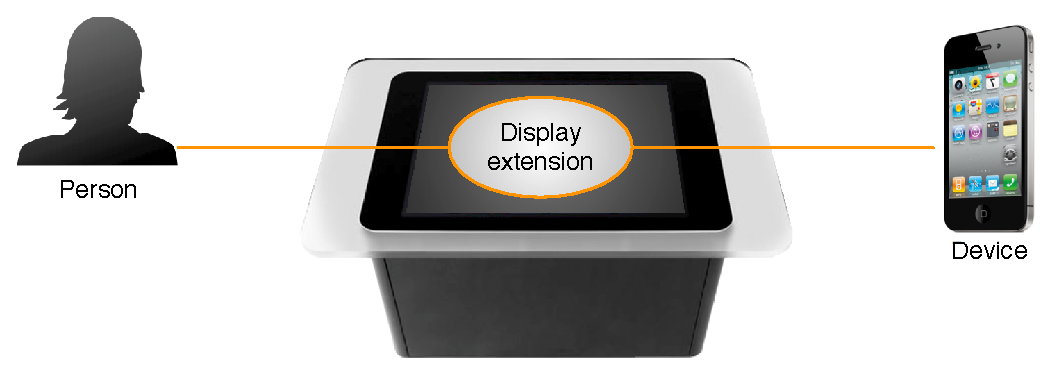
\includegraphics[width=0.9\textwidth]{images/useCase}
    \caption{Main use case.}
    \label{fig:useCase}
\end{figure}

\subsection{The devices}

\subsubsection{Tabletops}

A tabletop presents a range of characteristics that have concrete implications on the system design.
A tabletop is \ldots
\begin{description}

\item[\ldots a computer.] This project investigates a strategy where a tabletop is used as a smart IO peripheral.
The system should allow a tabletop to function as a relay between a personal device and users, forwarding both input and output as required.

\item[\ldots a table.] Its working surface is horizontal by nature, with the implication that it cannot support any prolonged interaction, because of the bad ergonomics of the ``hunched over'' working position.
Furthermore, a table gives naturally rise to various activities, such as eating, and it supports all sorts of objects, often in a collocated collaborative atmosphere.
The system should therefore support simultaneous users, and handle limited space availability.
Finally, a table offers no specific orientation, implying that the orientation of the system UI will have to adapt to the user's position around the tabletop.

\item[\ldots a situated device.] A tabletop is not mobile.
It usually sits at a specific location, and users come to it in order to use it.
The main implication is that tabletops seem to naturally fit in public spaces, where they are shared among multiple users.
This tendency is accentuated by the price factor, that makes a private person not likely to buy such a device for private use.
The system should handle public use, characterized by short anonymous sessions and an often interrupted interaction flow.
Other scenarios should be considered as well, such as a tabletop in an individual office, or in a family home.
In any case, it can be expected to have dedicated power supply and network connection, removing such concerns from the developer's mind.

\item[\ldots a shared device.] In many cases the tabletop will be shared by multiple users, raising concerns of user identification and data protection.

\item[\ldots an interactive surface.] As such, it typically offers large graphical output, as well as a range of input techniques to allow for user interaction.
Most tabletops support multitouch-based input.
This introduces a new kind of interaction model, more intuitive, that the system should be based upon.
In some cases, such as with camera-based devices, it is possible to add tangible objects to the tabletop experience.
This project will report on the possibilities to use a personal device as a tangible control integrated to the tabletop.

\end{description}

\subsubsection{Mobile computing devices}

A mobile computing device is \ldots

\begin{description}

\item[\ldots a computer.] It offers enough computing power, storage space and connectivity to support most users' daily tasks. The system should allow the user to access his/her applications and personal data.

\item[\ldots a small device.] Hence the mobility. Such a device is carried around by users. However, the small form factor implies a suboptimal graphical user experience.
The system should try to improve this, by offering superior IO resources.

\item[\ldots a mobile device.] With the implications that its power supply is limited by battery life, and its connectivity is unstable. The system should be developed with those concerns in mind.

\end{description}

\subsection{The situations}

There exists different types of everyday situations in which the system can be put to use.
They vary depending on whether they involve one or more users, and whether the tabletop is a public or private device.
A tabletop is considered a public device as soon as there are more than one user that have access to it.
As a consequence, the scenario of multiple users on a private tabletop is not considered.
Each situation implies a slightly different set of application features.
The original scenarios are included in appendix \ref{scenarios}.

\subsubsection{Single user on a public tabletop}

It should be possible for the user to wirelessly pair his/her personal device with a public tabletop computer.
This implies that the devices are both connected to the local wireless networks, that they are able to detect each other and discover each other's identity on the network.
It would not be safe to establish this connection automatically in a public space.
Therefore, dialogs should be used both on the mobile device and on the tabletop to gather user input.
The UI of the mobile device should be transferred to the interactive surface as graphical output, and this transferred display should be able to accept touch input to be forwarded back to the device.
The transferred display should be contained in an application window, and this window should be manipulable (drag, resize, rotate, minimize, hide, ..).

The application window should react to the state of the interactive surface.
An example of this is that the application window should turn inactive if it is obstructed by an object on the table.

Finally, the mobile device could be a participant in the interaction model, i.e. listing it off the table should interrupt the connection and exit the application.

%\begin{itemize}
%\item{the mobile device is automatically detected by the tabletop}
%\item{dialog windows are displayed on both devices}
%\item{the wireless connection is automatic}
%\item{the mobile device UI is transferred to the surface.}
%\item{the transferred UI can be resized, rotated and moved on the surface}
%\item{the transferred UI goes inactive when objects obstruct it}
%\item{user input is forwarded to the mobile device}
%\item{the transferred UI can be minimized and restored}
%\item{the application can be exited by lifting the mobile device off the table.}
%\end{itemize}

\subsubsection{Multi users on a public tabletop}

In a collocated collaborative context, it should be possible for more than one personal device to simultaneously have their display extended to the interactive surface.
This implies that the implementation should support parallel connections and simultaneous use.

Mobile computing devices come in many forms, and ideally the system should support all of them.
Devices vary in terms of software and hardware specifications.
Some parameters that are especially important here are the programming platform, as well as the display resolution.

When a tabletop is used simultaneously by multiple users, there is a very concrete risk of lack of space on the surface.
This fact introduces a new need for the system, to allow a user to remove his/her personal device from the table, while keeping the display extension active.

\subsubsection{Single user on a private tabletop}

If the tabletop is private, such as a home computer or a working desk, the system should offer extended functionalities to the user.
He/she should have the option to configure the tabletop in order to allow/initiate those extended functionalities.
Some suggested functionalities are:
\begin{itemize}
\item automatic launch of the display extension application
\item push application widgets from the extended display to the tabletop
\item share data between the personal device and the tabletop
\end{itemize}

\section{Solution requirements}

\subsection{Detection and pairing}



 system setup on the personal device

 discovery and pairing protocol

\subsection{UI transfer}

 UI output transfer to the tabletop

 UI input transfer to the personal device

\subsection{Surface UI}

 manipulation of the UI extension on the tabletop (drag, resize, rotate)

 minimize and restore of the UI extension

 support the personal device's physical buttons' functions

 switch display orientation on the UI extension

 handle obstruction of the UI extension

 push application widgets to the tabletop

\subsection{Tangible UI}

 UI extension attach/detach to the personal device on tabletop

 control the UI extension with the personal device (move UI, exit application)

\section{Interaction design}

\subsection{Storyboards}

After identifying system features, storyboards are the next step in the design process.
They are a more concrete design approach, and help defining the features in further details.
During this phase, the designer starts considering the graphical aspects of the system.

As an example, let us consider the action of resizing the UI extension.
This action is in effect one of the main points of interest of the system, as it allows a person to use her device on a potentially much larger screen.
Therefore, the resizing feature strikes as a necessary one.
Logically, the feature is included in a storyboard.
Thus, a UI element must be defined that implements it.
At this point, different solutions come up, such as using 2 fingers to pull the window apart, or dragging a corner down to make the window larger.
\\\\
INCLUDE STORYBOARD EXCERPT
\\\\
Storyboards help generating design options.

\subsection{Generating ideas with low fidelity prototypes}

%\begin{figure}[h!]
%  \caption{Low fidelity prototypes.}
%  \centering
%    \includegraphics[width=0.8\textwidth]{images/paperprot1}
%\end{figure}
%
%\begin{figure}[h!]
%  \caption{Low fidelity prototypes.}
%  \centering
%    \includegraphics[width=0.8\textwidth]{images/paperprot2}
%\end{figure}
%
%\begin{figure}[h!]
%  \caption{Low fidelity prototypes.}
%  \centering
%    \includegraphics[width=0.8\textwidth]{images/paperprot3}
%\end{figure}

\subsection{Commands and actions}

Human computer interaction can be modeled as a simple cause-effect relationship.

The user wishes the computer to execute a command.
To achieve that, he/she performs an action, making use of the available input devices (keyboard, mouse, etc..) and interfaces.
The action is the cause, the command is the effect, and together they form a single interaction between user and machine.

On an interactive surface, the traditional input devices are gone, and the interaction is based on hand gestures.

Those concepts are inspired by the paper ``User-Defined Gestures for Surface Computing'' by Wobbrock, \citep{Wobbrock:2009:gestures}.

The following six basic commands (interaction primitives) were identified and progressively chosen as being essential to the TableIO application.

\begin{enumerate}
\item{\emph{Dragging} the application window across the interactive surface.}
\item{\emph{Rotating} the application window across the interactive surface.}
\item{\emph{Resizing} the application window across the interactive surface.}
\item{\emph{Minimizing} the application window, making it possible to restore it easily.}
\item{\emph{Hiding} the content of the application window.}
\item{\emph{Exiting} the application, thus closing the application window.}
\end{enumerate}

EXTRA command: device buttons (HOME on the iPhone) should be supported.

\subsection{Interaction strategies}

Various interaction techniques can be used to invoke application level commands.

Early idea generation process lead to the definition of  specific interaction strategies.

Each strategy can be consistently implemented for each previously defined command.

\begin{enumerate}
\item{\emph{Action Tabs} are traditional buttons/tabs that implement functionalities.}
\item{The \emph{Action Bar} can be compared to a virtual touchpad, it includes a manipulation area and buttons.}
\item{\emph{Window Toggle} refers to using a switch to toggle the window between inactive and active states. In its inactive state, the window is made manipulable as a common digital picture.}
\item{The \emph{Active Border} is a digital frame around the application window used for manipulation.}
\item{\emph{Active Corners} is a strategy similar to Active Border, with the difference that the border's corners implement specific functionalities.}
\item{\emph{Other} regroups suggestions that do not fit with any specific strategy.}
\end{enumerate}

\section{Preliminary usability study}

A well-designed product is a successful one.
Usability and appeal are key elements towards the success of an application.
The goal of this experiment is to gather knowledge directly from users to inform important design decisions.

Example of designers designs that fails from user standpoint.

The goal is to have potential users of the system describe their ideal user interface.

The focus of the experiment is not the interaction with the mirrored smartphone's screen.
The focus is the manipulation of the application window that contains the mirrored display.

\subsection{Method}	

\subsubsection{Parameters}

The parameters of the experiment are the above mentioned commands and actions.
The 6 commands form a set of features that are considered necessary for the application to function.

For each of the chosen commands, we have 6 implementation suggestions (1 for each interaction strategy).

\subsubsection{Participants}


\subsubsection{Experiment}

The experiment is based on low fidelity prototypes.
Instead of a digital user interface, the participant interacts with paper representations.

The user is asked to perform a task using the application.
The task is divided into the 6 actions that 


\subsection{Results}

\section{Design Choices}

Comments:
users suggest dragging/rotating the window directly (forget that window forwards input to device)

LIMITS:
UNFORTUNATELY, results are biased due to splitting the suggestions in 2, for each participant group.
Ranking result for 1 strategy is only valid compared to 2 other suggestions from same participant group, not valid across all strategies.

focus on coherence of interaction

move from traditional explicit buttons towards a more implicit, physical interaction.

Interest of playful, exploratory learning process for the user

Interest of appealing design

\subsection{users best}

\subsection{designers best}

\subsection{hybrid}


\begin{figure}[]
  \caption{Interaction primitives.}
  \centering
    \includegraphics[]{images/primHistog}
\end{figure}

\begin{figure}[]
  \caption{Interaction strategies.}
  \centering
    \includegraphics[]{images/stratHistog}
\end{figure}

